\chapter{In het atoom}\label{ch:g9:inside-the-atom}

In 1909 werd in een laboratorium in Manchester een bundel piepkleine,
snelle deeltjes afgevuurd op een vel bladgoud van een paar honderd \omterm{def:g7:atoms-and-molecules:atom}{atomen}
dik. Bijna alle deeltjes gingen er recht doorheen, alsof het goud leeg
was. Maar ongeveer één op enkele duizenden kaatste terug. ``Het was
alsof je een granaat van vijftien inch afvuurde op een vel vloeipapier
en die terugkwam en jou raakte,'' zei Ernest Rutherford, wiens studenten
het experiment hadden uitgevoerd. Het \omterm{def:g7:atoms-and-molecules:atom}{atoom}, het ondeelbare stukje
materie, had een opbouw --- en het was bijna helemaal leeg.

\begin{recall}
Alle materie bestaat uit \omterm{def:g7:atoms-and-molecules:atom}{atomen}, waarvan er ongeveer honderd soorten
zijn, elk met een symbool zoals \ce{H}, \ce{C}, \ce{O}, \ce{Fe}. \omterm{def:g7:atoms-and-molecules:atom}{Atomen}
verbinden zich tot \omterm{def:g7:atoms-and-molecules:molecule}{moleculen}, die je beschrijft met formules zoals
\ce{H2O} (\cref{ch:g7:atoms-and-molecules}).
\end{recall}

\section{Kern en elektronen}

\begin{definition}[Atoomkern en elektron]\label{def:g9:inside-the-atom:nucleus}
Elk \omterm{def:g7:atoms-and-molecules:atom}{atoom} heeft een piepklein, zwaar binnenste, de
\emph{atoomkern}\index{atoomkern}, die een positieve elektrische lading
draagt. Daaromheen bewegen veel lichtere deeltjes, de
\emph{elektronen}\index{elektron}, die elk dezelfde negatieve lading
dragen, $-e$.
\end{definition}

\begin{proposition}[Een atoom is neutraal]\label{prop:g9:inside-the-atom:neutral}
% ledger: const:e
Een \omterm{def:g7:atoms-and-molecules:atom}{atoom} als geheel draagt geen elektrische lading: de positieve lading
van zijn kern wordt precies opgeheven door de negatieve ladingen van zijn
\omterm{def:g9:inside-the-atom:nucleus}{elektronen}. De lading $e$ is piepklein: $e = \qty{1.60e-19}{C}$ (de
coulomb, de eenheid van lading, hoort bij het natuurkundeboek).
\end{proposition}

\begin{omfigure}
\begin{tikzpicture}[font=\small]
  \shade[inner color=omDef!35, outer color=white] (0,0) circle (2.2);
  \draw[omDef!60, dashed] (0,0) circle (2.2);
  \foreach \a/\r in {20/1.6,95/1.1,150/1.9,215/1.4,290/1.7,340/0.9} {
    \fill[omDef] (\a:\r) circle (0.06);
    \node[font=\scriptsize, omDef] at ($(\a:\r)+(0.18,0.16)$) {$-$};
  }
  \fill[red!70!black] (0,0) circle (0.1);
  \draw[<-, omProp, thick] (-0.12,0.02) -- (-3.0,0.9) node[left, text=black, align=right]
    {kern: piepklein,\\ zwaar, positief};
  \draw[<-, omProp, thick] ($(20:1.6)+(0.08,0.02)$) -- (3.0,0.9) node[right, text=black]
    {een elektron: licht, negatief};
  \draw[<-, omProp, thick] (300:2.2) -- (3.0,-1.4) node[right, text=black, align=left]
    {de elektronen bewegen in een wolk\\ rond de kern};
\end{tikzpicture}

{\small Een \omterm{def:g7:atoms-and-molecules:atom}{atoom}, niet op schaal. Als je de kern zo groot tekende als
het rode puntje, zou de elektronenwolk een paar honderd meter breed zijn.}
\end{omfigure}

\section{Protonen en neutronen}

\begin{definition}[Proton, neutron, nucleon]\label{def:g9:inside-the-atom:proton}
De kern bestaat uit twee soorten deeltjes: \emph{protonen}\index{proton},
die elk de lading $+e$ dragen, en \emph{neutronen}\index{neutron}, die
geen lading dragen. Protonen en neutronen, die bijna dezelfde massa
hebben, heten samen \emph{nucleonen}\index{nucleon}.
\end{definition}

\begin{definition}[Atoomnummer en massagetal]\label{def:g9:inside-the-atom:atomic-number}
Het aantal \omterm{def:g9:inside-the-atom:proton}{protonen} in een kern is het
\emph{atoomnummer}\index{atoomnummer}, geschreven als $Z$. Het aantal
\omterm{def:g9:inside-the-atom:proton}{nucleonen} (\omterm{def:g9:inside-the-atom:proton}{protonen} en \omterm{def:g9:inside-the-atom:proton}{neutronen} samen) is het
\emph{massagetal}\index{massagetal}, geschreven als $A$. Het aantal
\omterm{def:g9:inside-the-atom:proton}{neutronen} is $N = A - Z$.
\end{definition}

\begin{notation}[Het nuclidesymbool]\label{not:g9:inside-the-atom:symbol}
Een \omterm{def:g7:atoms-and-molecules:atom}{atoom} met een bepaalde kern schrijf je met zijn symbool, het
\omterm{def:g9:inside-the-atom:atomic-number}{massagetal} linksboven en het \omterm{def:g9:inside-the-atom:atomic-number}{atoomnummer} linksonder:
\ce{^{A}_{Z}X}. Zo heeft \ce{^{12}_{6}C} 6 \omterm{def:g9:inside-the-atom:proton}{protonen} en $12 - 6 =
6$ \omterm{def:g9:inside-the-atom:proton}{neutronen}; \ce{^{56}_{26}Fe} heeft 26 \omterm{def:g9:inside-the-atom:proton}{protonen} en 30 \omterm{def:g9:inside-the-atom:proton}{neutronen}.
\end{notation}

\begin{method}[Een nuclidesymbool lezen]\label{met:g9:inside-the-atom:read}
Voor \ce{^{A}_{Z}X}:
\begin{enumerate}
  \item \omterm{def:g9:inside-the-atom:proton}{protonen}: $Z$;
  \item \omterm{def:g9:inside-the-atom:proton}{neutronen}: $A - Z$;
  \item \omterm{def:g9:inside-the-atom:nucleus}{elektronen} van het neutrale \omterm{def:g7:atoms-and-molecules:atom}{atoom}: $Z$, evenveel als \omterm{def:g9:inside-the-atom:proton}{protonen}.
\end{enumerate}
Voor \ce{^{23}_{11}Na}: 11 \omterm{def:g9:inside-the-atom:proton}{protonen}, 12 \omterm{def:g9:inside-the-atom:proton}{neutronen}, 11 \omterm{def:g9:inside-the-atom:nucleus}{elektronen}.
\end{method}

\begin{omfigure}
\begin{tikzpicture}[font=\small]
  \node[font=\Huge, inner sep=1pt] (x) at (0,0) {\ce{^{35}_{17}Cl}};
  \draw[<-, omProp, thick, shorten <=3pt] ([xshift=5pt,yshift=-7pt]x.north west) -- (-2.6,1.0)
    node[left, text=black, align=right] {massagetal $A = 35$:\\ protonen + neutronen};
  \draw[<-, omProp, thick, shorten <=3pt] ([xshift=5pt,yshift=7pt]x.south west) -- (-2.6,-1.0)
    node[left, text=black, align=right] {atoomnummer $Z = 17$:\\ protonen};
  \draw[<-, omProp, thick] ([xshift=2pt]x.east) -- (2.2,0) node[right, text=black,
    align=left] {symbool van het element:\\ chloor};
\end{tikzpicture}

{\small Een nuclidesymbool lezen: dit chlooratoom heeft 17 \omterm{def:g9:inside-the-atom:proton}{protonen},
$35 - 17 = 18$ \omterm{def:g9:inside-the-atom:proton}{neutronen}, en als het neutraal is 17 \omterm{def:g9:inside-the-atom:nucleus}{elektronen}.}
\end{omfigure}

\section{Het chemisch element en zijn isotopen}

\begin{definition}[Chemisch element]\label{def:g9:inside-the-atom:element}
Een \emph{chemisch element}\index{chemisch element} is de verzameling
van alle \omterm{def:g7:atoms-and-molecules:atom}{atomen}, en van alle geladen \omterm{def:g7:atoms-and-molecules:atom}{atomen} die daaruit gemaakt zijn,
die hetzelfde \omterm{def:g9:inside-the-atom:atomic-number}{atoomnummer} $Z$ hebben. Elk element heeft een naam en een
symbool: elk \omterm{def:g7:atoms-and-molecules:atom}{atoom} met 6 \omterm{def:g9:inside-the-atom:proton}{protonen} is een koolstofatoom, \ce{C}; elk \omterm{def:g7:atoms-and-molecules:atom}{atoom}
met 8 \omterm{def:g9:inside-the-atom:proton}{protonen} is een zuurstofatoom, \ce{O}.
\end{definition}

\begin{definition}[Isotopen]\label{def:g9:inside-the-atom:isotope}
\omterm{def:g7:atoms-and-molecules:atom}{Atomen} van hetzelfde element die een verschillend aantal \omterm{def:g9:inside-the-atom:proton}{neutronen}
hebben, en dus een verschillend \omterm{def:g9:inside-the-atom:atomic-number}{massagetal}, zijn
\emph{isotopen}\index{isotoop} van dat element. Ze hebben dezelfde $Z$
en een verschillende $A$.
\end{definition}

\begin{example}[Isotopen van koolstof en van waterstof]\label{ex:g9:inside-the-atom:isotopes}
% ledger: iso:C12, iso:C13, iso:H2
Natuurlijke koolstof bestaat voor ongeveer \qty{98.9}{\percent} uit
koolstof-12, \ce{^{12}_{6}C}, en voor \qty{1.1}{\percent} uit koolstof-13,
\ce{^{13}_{6}C}, met een spoor koolstof-14, \ce{^{14}_{6}C}, waarvan de
langzame omzetting in een andere kern gebruikt wordt om oud hout en
botten te dateren (radioactiviteit hoort bij het natuurkundeboek).
Waterstof heeft drie \omterm{def:g9:inside-the-atom:isotope}{isotopen}: \ce{^{1}_{1}H}, helemaal zonder \omterm{def:g9:inside-the-atom:proton}{neutron},
verreweg het meest voorkomend; deuterium \ce{^{2}_{1}H}, een paar \omterm{def:g7:atoms-and-molecules:atom}{atomen}
op elke honderdduizend; en tritium \ce{^{3}_{1}H}.
\end{example}

\begin{proposition}[Isotopen gedragen zich chemisch hetzelfde]\label{prop:g9:inside-the-atom:alike}
De chemie van een \omterm{def:g7:atoms-and-molecules:atom}{atoom} hangt af van zijn \omterm{def:g9:inside-the-atom:nucleus}{elektronen}, en de \omterm{def:g9:inside-the-atom:isotope}{isotopen} van
een element hebben evenveel \omterm{def:g9:inside-the-atom:nucleus}{elektronen}. \omterm{def:g9:inside-the-atom:isotope}{Isotopen} reageren daarom op
dezelfde manier: water dat met deuterium gemaakt is, ziet er bijna
precies zo uit en gedraagt zich bijna precies zo als gewoon water.
\end{proposition}

\begin{omfigure}
\begin{tikzpicture}[font=\small, p/.style={circle, inner sep=0pt, minimum size=4.2mm,
    ball color=red!65}, n/.style={circle, inner sep=0pt, minimum size=4.2mm,
    ball color=black!20}]
  \node[p] at (0,0) {};
  \node[anchor=north, align=center] at (0,-0.45) {\ce{^{1}_{1}H}\\ 1 proton};
  \node[p] at (3.0,0) {}; \node[n] at (3.35,0.1) {};
  \node[anchor=north, align=center] at (3.2,-0.45) {\ce{^{2}_{1}H}\\ 1 proton, 1 neutron};
  \node[p] at (6.4,0) {}; \node[n] at (6.75,0.12) {}; \node[n] at (6.55,0.35) {};
  \node[anchor=north, align=center] at (6.6,-0.45) {\ce{^{3}_{1}H}\\ 1 proton, 2 neutronen};
  \node[draw=black!30, fill=red!65, circle, minimum size=3mm, inner sep=0pt] at (9.1,0.2) {};
  \node[anchor=west] at (9.3,0.2) {proton};
  \node[draw=black!30, fill=black!20, circle, minimum size=3mm, inner sep=0pt] at (9.1,-0.3) {};
  \node[anchor=west] at (9.3,-0.3) {neutron};
\end{tikzpicture}

{\small De kernen van de drie \omterm{def:g9:inside-the-atom:isotope}{isotopen} van waterstof: elk één \omterm{def:g9:inside-the-atom:proton}{proton}, en
0, 1 of 2 \omterm{def:g9:inside-the-atom:proton}{neutronen}.}
\end{omfigure}

\section{Afmetingen en massa's}

\begin{proposition}[De kern is piepklein en bevat bijna alle massa]\label{prop:g9:inside-the-atom:sizes}
% ledger: const:a0, r:proton, const:mp, const:mn, const:me
Een \omterm{def:g7:atoms-and-molecules:atom}{atoom} is ongeveer \qty{e-10}{m} breed; zijn kern ongeveer
\qty{e-15}{m} tot \qty{e-14}{m}: zo'n tienduizend tot honderdduizend keer
kleiner. De massa's van de deeltjes zijn
\[
  m_p = \qty{1.673e-27}{kg},\qquad m_n = \qty{1.675e-27}{kg},\qquad
  m_e = \qty{9.11e-31}{kg}.
\]
Een \omterm{def:g9:inside-the-atom:proton}{proton} is ongeveer 1836 keer zwaarder dan een \omterm{def:g9:inside-the-atom:nucleus}{elektron}, dus meer dan
\qty{99.9}{\percent} van de massa van een \omterm{def:g7:atoms-and-molecules:atom}{atoom} zit in zijn kern.
\end{proposition}

\begin{example}[Een knikker in een stadion]\label{ex:g9:inside-the-atom:marble}
Als de kern van een \omterm{def:g7:atoms-and-molecules:atom}{atoom} een knikker van \qty{1}{cm} was, zou het \omterm{def:g7:atoms-and-molecules:atom}{atoom}
ongeveer $\qty{1}{cm} \times 100\,000 = \qty{1}{km}$ breed zijn: een
knikker midden in een reusachtig stadion, met een paar stofjes --- de
\omterm{def:g9:inside-the-atom:nucleus}{elektronen} --- die rond de tribunes wervelen. Materie is grotendeels
lege ruimte.
\end{example}

\begin{method}[De massa van een atoom]\label{met:g9:inside-the-atom:mass}
Omdat \omterm{def:g9:inside-the-atom:proton}{protonen} en \omterm{def:g9:inside-the-atom:proton}{neutronen} bijna dezelfde massa hebben en \omterm{def:g9:inside-the-atom:nucleus}{elektronen}
heel licht zijn, ligt de massa van een \omterm{def:g7:atoms-and-molecules:atom}{atoom} dicht bij $A \times
\qty{1.67e-27}{kg}$, waarbij $A$ het \omterm{def:g9:inside-the-atom:atomic-number}{massagetal} is. Een koolstof-12-atoom:
$12 \times 1.67 \times 10^{-27} = \qty{2.00e-26}{kg}$.
\end{method}

\section{Een korte geschiedenis van het atoommodel}

\begin{history}[Van het ondeelbare tot de kern, 1897--1932]
In 1897 ontdekte J.~J.~Thomson het \omterm{def:g9:inside-the-atom:nucleus}{elektron}, een deeltje dat veel lichter
is dan welk \omterm{def:g7:atoms-and-molecules:atom}{atoom} ook: \omterm{def:g7:atoms-and-molecules:atom}{atomen} waren dus toch deelbaar. Hij stelde zich
het \omterm{def:g7:atoms-and-molecules:atom}{atoom} voor als een bol positieve materie met \omterm{def:g9:inside-the-atom:nucleus}{elektronen} erin, als
krenten in een bol. In 1909--1911 liet het goudfolie-experiment van het
team van Rutherford zien dat de positieve lading en bijna alle massa in
een piepkleine kern zitten. In 1913 stelde Niels Bohr voor dat de
\omterm{def:g9:inside-the-atom:nucleus}{elektronen} vaste energieniveaus rond die kern bezetten, en in 1932 vond
James Chadwick het \omterm{def:g9:inside-the-atom:proton}{neutron}.
\end{history}

\begin{omfigure}
\begin{minipage}[b]{0.3\linewidth}\centering
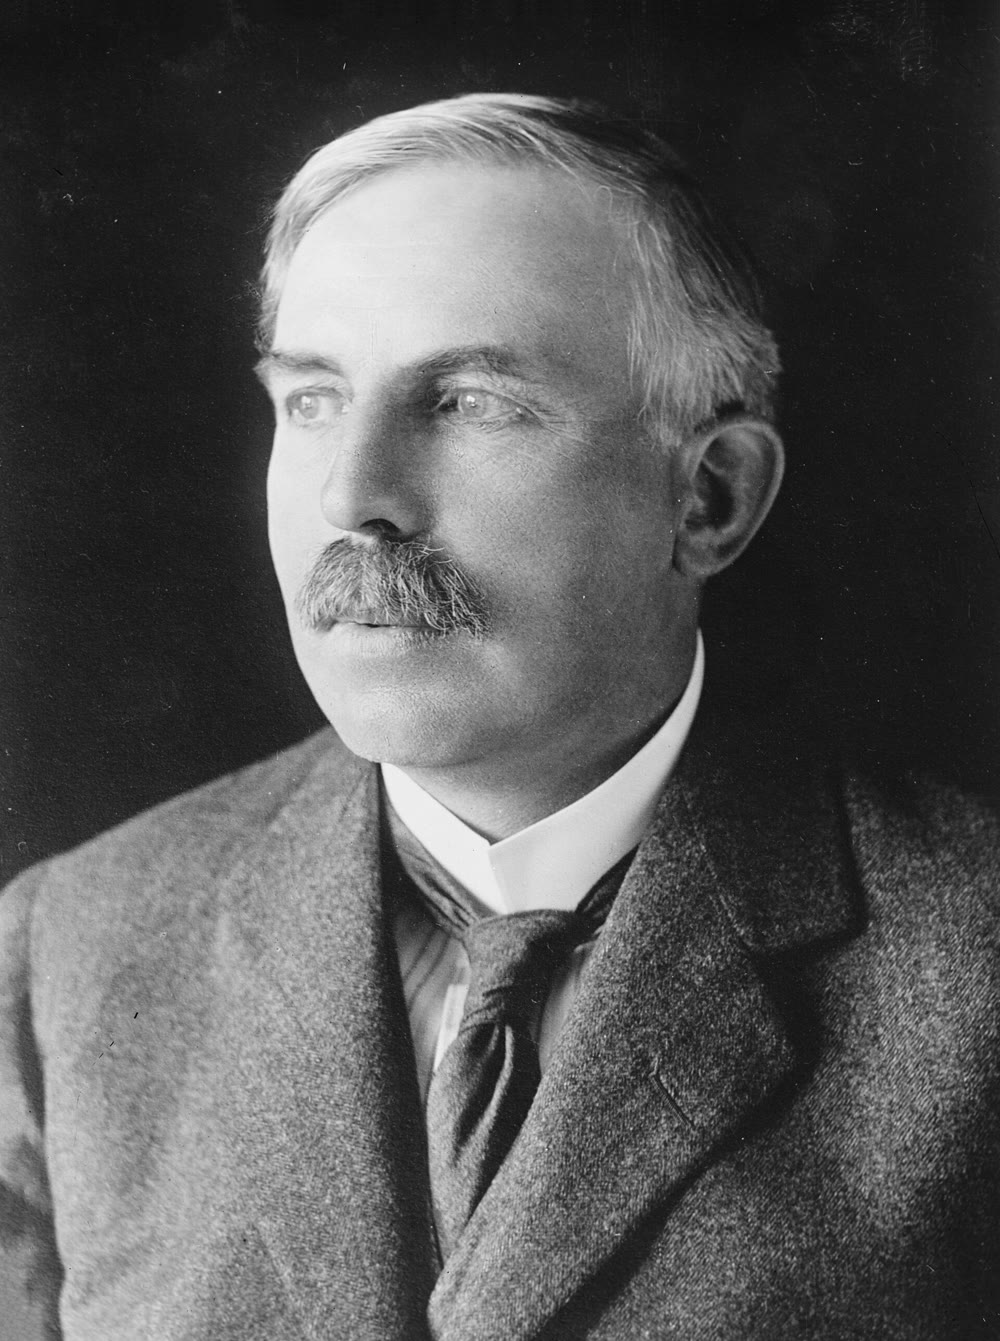
\includegraphics[width=\linewidth]{images/book1/rutherford.jpg}

{\small Ernest Rutherford (1871--1937).}
\end{minipage}\hfill
\begin{minipage}[b]{0.66\linewidth}\centering
\begin{tikzpicture}[font=\small]
  \fill[black!45] (0,-0.5) rectangle (0.9,0.5);
  \node[anchor=north, align=center] at (0.45,-0.55) {bron van\\ alfadeeltjes};
  \draw[->, thick, red!70!black] (0.9,0) -- (2.8,0);
  \fill[yellow!70!orange] (2.8,-1.6) rectangle (2.88,1.6);
  \node[anchor=north] at (2.84,-1.65) {bladgoud};
  \draw[omDef!40, line width=4pt] (5.6,-1.8) arc[start angle=-30, end angle=30, radius=3.6];
  \foreach \y in {-0.3,-0.1,0.1,0.3} \draw[->, red!70!black] (2.88,\y) -- (5.3,\y);
  \draw[->, red!70!black] (2.88,0.05) -- (5.0,1.15);
  \draw[->, red!70!black] (2.88,-0.05) -- (4.9,-1.3);
  \draw[->, red!70!black, thick] (2.8,0.02) .. controls (2.2,0.35) .. (1.6,0.95);
  \node[anchor=west, align=left, font=\footnotesize] at (6.25,0) {de meeste\\ gaan recht\\ door};
  \node[anchor=south, align=center, font=\footnotesize] at (1.6,1.0) {heel enkele\\ kaatsen terug};
\end{tikzpicture}

{\small Het goudfolie-experiment: de meeste deeltjes gaan recht door; een
paar worden afgebogen; heel enkele kaatsen terug op een kern.}
\end{minipage}
\end{omfigure}

\section{Oefeningen}

\begin{exercise}[$\star$]\label{exo:g9:inside-the-atom:1}
Noem de deeltjes van de kern en de deeltjes eromheen, met het teken van
hun lading.
\end{exercise}

\begin{exercise}[$\star$]\label{exo:g9:inside-the-atom:2}
Geef het aantal \omterm{def:g9:inside-the-atom:proton}{protonen}, \omterm{def:g9:inside-the-atom:proton}{neutronen} en \omterm{def:g9:inside-the-atom:nucleus}{elektronen} van \ce{^{16}_{8}O},
\ce{^{27}_{13}Al} en \ce{^{40}_{20}Ca}.
\end{exercise}

\begin{exercise}[$\star$]\label{exo:g9:inside-the-atom:3}
Waarom is een \omterm{def:g7:atoms-and-molecules:atom}{atoom} elektrisch neutraal?
\end{exercise}

\begin{exercise}[$\star$]\label{exo:g9:inside-the-atom:4}
Een \omterm{def:g7:atoms-and-molecules:atom}{atoom} heeft 26 \omterm{def:g9:inside-the-atom:proton}{protonen} en 30 \omterm{def:g9:inside-the-atom:proton}{neutronen}. Schrijf zijn nuclidesymbool
op (het element is ijzer, \ce{Fe}).
\end{exercise}

\begin{exercise}[$\star\star$]\label{exo:g9:inside-the-atom:5}
Zijn \ce{^{35}_{17}Cl} en \ce{^{37}_{17}Cl} hetzelfde element? Zijn het
\omterm{def:g9:inside-the-atom:isotope}{isotopen}? Leg uit.
\end{exercise}

\begin{exercise}[$\star\star$]\label{exo:g9:inside-the-atom:6}
Zijn \ce{^{14}_{6}C} en \ce{^{14}_{7}N} \omterm{def:g9:inside-the-atom:isotope}{isotopen}? Leg uit.
\end{exercise}

\begin{exercise}[$\star\star$]\label{exo:g9:inside-the-atom:7}
Bereken, in wetenschappelijke notatie, de massa bij benadering van een
\omterm{def:g7:atoms-and-molecules:atom}{atoom} \ce{^{56}_{26}Fe}.
\end{exercise}

\begin{exercise}[$\star\star$]\label{exo:g9:inside-the-atom:8}
Waarom gaan bij het goudfolie-experiment de meeste deeltjes recht door
het goud heen?
\end{exercise}

\begin{exercise}[$\star\star$]\label{exo:g9:inside-the-atom:9}
Hoeveel keer kleiner dan een \omterm{def:g7:atoms-and-molecules:atom}{atoom} (\qty{e-10}{m}) is een kern van
\qty{e-15}{m}? Schrijf het antwoord als een macht van tien.
\end{exercise}

\begin{exercise}[$\star\star$]\label{exo:g9:inside-the-atom:10}
Waarom hebben de \omterm{def:g9:inside-the-atom:isotope}{isotopen} van een element dezelfde chemie?
\end{exercise}

\begin{exercise}[$\star\star\star$]\label{exo:g9:inside-the-atom:11}
Een ijzeratoom heeft 26 \omterm{def:g9:inside-the-atom:nucleus}{elektronen}. Bereken hun totale massa, en daarna
welk deel van de massa van een \omterm{def:g7:atoms-and-molecules:atom}{atoom} \ce{^{56}_{26}Fe} ze uitmaken
(gebruik de massa uit oefening~7).
\end{exercise}

\begin{exercise}[$\star\star\star$]\label{exo:g9:inside-the-atom:12}
% ledger: iso:Cu63, iso:Cu65
Natuurlijk koper bestaat voor \qty{69.15}{\percent} uit koper-63 en voor
\qty{30.85}{\percent} uit koper-65. Hoeveel \omterm{def:g7:atoms-and-molecules:atom}{atomen} van elke \omterm{def:g9:inside-the-atom:isotope}{isotoop} zijn
er op 10\,000 koperatomen? Wat is het gemiddelde aantal \omterm{def:g9:inside-the-atom:proton}{nucleonen} per
koperatoom?
\end{exercise}

\clearpage % houdt de kop bij het kader van het probleem (hij bleef onderaan een pagina achter)
\section{Probleem: Chloor wegen}

\begin{problem}[{Weekendprobleem --- twee isotopen van chloor, de massa
van elk atoom, en de gemiddelde massa van een chlooratoom}]
\label{pb:g9:inside-the-atom:1}
% ledger: iso:Cl35, iso:Cl37, const:me, const:mp, const:mn
Natuurlijk chloor is een \omterm{def:g6:pure-substances-and-mixtures:mixture}{mengsel} van twee \omterm{def:g9:inside-the-atom:isotope}{isotopen}, chloor-35 en
chloor-37: van elke 1000 chlooratomen zijn er ongeveer 758 chloor-35 en
242 chloor-37. Neem voor de massa van een \omterm{def:g9:inside-the-atom:proton}{nucleon} \qty{1.67e-27}{kg} en
voor de massa van een \omterm{def:g9:inside-the-atom:nucleus}{elektron} \qty{9.11e-31}{kg}. Het \omterm{def:g9:inside-the-atom:atomic-number}{atoomnummer} van
chloor is 17.

\medskip
\noindent\textbf{Deel I --- Twee kernen.}
\begin{enumerate}
  \item Schrijf de nuclidesymbolen van de twee \omterm{def:g9:inside-the-atom:isotope}{isotopen} op.
  \item Geef van elk het aantal \omterm{def:g9:inside-the-atom:proton}{protonen}, \omterm{def:g9:inside-the-atom:proton}{neutronen} en \omterm{def:g9:inside-the-atom:nucleus}{elektronen}.
  \item Waarom heten ze allebei chloor? Waarom zijn het \omterm{def:g9:inside-the-atom:isotope}{isotopen}?
  \item Reageert een monster chloor-37 op dezelfde manier met natrium als
        een monster chloor-35? Leg uit.
\end{enumerate}

\medskip
\noindent\textbf{Deel II --- De massa van elk \omterm{def:g7:atoms-and-molecules:atom}{atoom}.}
\begin{enumerate}[resume]
  \item Bereken de massa van de kern van een chloor-35-atoom.
  \item Bereken de massa van de 17 \omterm{def:g9:inside-the-atom:nucleus}{elektronen}, en controleer dat je die
        naast de kern mag verwaarlozen.
  \item Bereken de massa van een chloor-37-atoom.
  \item Hoeveel chloor-35-atomen zouden samen \qty{1}{g} wegen? Geef het
        antwoord in wetenschappelijke notatie.
\end{enumerate}

\medskip
\noindent\textbf{Deel III --- Het gemiddelde \omterm{def:g7:atoms-and-molecules:atom}{atoom}.}
\begin{enumerate}[resume]
  \item Welk percentage van de chlooratomen is chloor-35? En chloor-37?
  \item Bereken voor 1000 \omterm{def:g7:atoms-and-molecules:atom}{atomen} natuurlijk chloor de totale massa van de
        chloor-35-atomen en van de chloor-37-atomen.
  \item Bereken de massa van deze 1000 \omterm{def:g7:atoms-and-molecules:atom}{atomen}.
  \item Leid daaruit de gemiddelde massa van een chlooratoom af.
\end{enumerate}
\end{problem}
